%--------------------------------------------------------------------
% NE 155 (intro to numerical simulation of radiation transport)
% Spring 2015

% formatting
\documentclass[12pt]{article}
\usepackage[top=1in, bottom=1in, left=1in, right=1in]{geometry}

\usepackage{setspace}
\onehalfspacing

\setlength{\parindent}{0mm} \setlength{\parskip}{1em}


% packages
\usepackage{amssymb}
%% The amsthm package provides extended theorem environments
\usepackage{amsthm}
\usepackage{epsfig}
\usepackage{times}
\renewcommand{\ttdefault}{cmtt}
\usepackage{amsmath}
\usepackage{graphicx} % for graphics files

% Draw figures yourself
\usepackage{tikz} 

% The float package HAS to load before hyperref
\usepackage{float} % for psuedocode formatting
\usepackage{xspace}

% from Denovo methods manual
\usepackage{mathrsfs}
\usepackage[mathcal]{euscript}
\usepackage{color}
\usepackage{array}

\usepackage[pdftex]{hyperref}

\newcommand{\nth}{n\ensuremath{^{\text{th}}} }
\newcommand{\ve}[1]{\ensuremath{\mathbf{#1}}}
\newcommand{\macro}{\ensuremath{\Sigma}}
\newcommand{\vOmega}{\ensuremath{\hat{\Omega}}}

\newcommand{\cc}[1]{\ensuremath{\overline{#1}}}
\newcommand{\ccm}[1]{\ensuremath{\overline{\mathbf{#1}}}}


%--------------------------------------------------------------------
%--------------------------------------------------------------------
\begin{document}
\begin{center}
{\bf NE 155, Classes 23-14, S16 \\
Finite Difference and Volume Methods for the Eigenvalue form of the DE \\ March 14 \& 16, 2016}
\end{center}

\setlength{\unitlength}{1in}
\begin{picture}(6,.1) 
\put(0,0) {\line(1,0){6.25}}         
\end{picture}

%--------------------------------------------------------------------
\section*{Finite Difference Method, Eigenvalue Problem}

We can extend all of the finite difference and finite volume methods we just learned to the eigenvalue problem case, which is another layer of complication. 

Now instead of a fixed source, we have an eigenvalue problem
\[-\frac{d}{dx}D(x)\frac{d \phi(x)}{dx} + \Sigma_a(x) \phi(x) = \frac{1}{k}\nu \Sigma_f(x) \phi(x) \]
%
\begin{figure}[h!]
\begin{center}
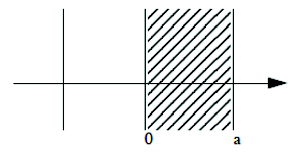
\includegraphics[height=1in]{FVM-fig}
\end{center}
\end{figure}
%
Let's again have a reflecting condition at the centerline ($x_0 = 0$) and vacuum on the right ($x_n = a$):
\begin{align}
\frac{d}{dx}\phi(x) \big|_{x=0} &= 0 \qquad \text{zero net current,} \nonumber\\
\phi(\tilde{a}) &= 0 \qquad \tilde{a} = a + 2D\:. \nonumber
\end{align}
%
We again have a spatial mesh:
%
\begin{center}
\begin{tikzpicture}
\draw (-.25,0)--(1.25,0);
\draw[dotted] (1.25,0)--(2.75,0);
\draw (2.75,0)--(5.25,0);
\draw[dotted] (5.25,0)--(6.75,0);
\draw (6.75,0)--(8.25,0);
%\draw (4,0)--(5.25,0);
\draw (0,-.25)--(0,.25);
\draw (1,-.25)--(1,.25);
%\draw (2,-.25)--(2,.25);
\draw (3,-.25)--(3,.25);
\draw (4,-.25)--(4,.25);
\draw (5,-.25)--(5,.25);
\draw (7,-.25)--(7,.25);
\draw (8,-.25)--(8,.25);
\node[below] at (0,-.25) {$x_0$};
\node[below] at (1,-.25) {$x_1$};
\node[below] at (3,-.25) {$x_{i-1}$};
\node[below] at (4,-.25) {$x_i$};
\node[below] at (5,-.25) {$x_{i+1}$};
\node[below] at (7,-.25) {$x_{n-1}$};
\node[below] at (8,-.25) {$x_n$};
\node[above] at (0.5, 0.5) {$h_1$};
\node[above] at (3.5, 0.5) {$h_i$};
\end{tikzpicture}
\end{center}
%
and in this configuration $x_0 = 0$, $x_n = a$, and $h_i$ is the mesh spacing. There are $n+1$ points and $n$ mesh cells.

Material discontinuities will coincide with the cell \textit{edges}, $x_i$. Thus, we can assume that the cross sections and the diffusion coefficient are constant in each cell:
%
%\begin{align}
%D(x) &= D_i \qquad \text{for } x_{i-1} \leq x \leq x_i \:,\nonumber \\
%\Sigma_{a}(x) &= \Sigma_{a,i} \qquad \text{for } x_{i-1} \leq x \leq x_i \:, \nonumber \\
%\nu\Sigma_f(x) &= \nu\Sigma_{f,i}\;, \quad \text{for } x_{i-1} \leq x \leq x_i\:, \nonumber \\
%h_i &\equiv x_i - x_{i-1} \:.\nonumber 
%\end{align}
%
The unknown values are again defined at the mesh or cell \textit{edges}, e.g.\ $\phi(x_i) = \phi_i$.

We derive the equations just like we did in the fixed source case, but now instead of $S_i$ we have $\nu \Sigma_{f,i}$ on the rhs and a $1/k$ in multiplying the rhs vector.

\begin{align}
\frac{\phi_{i+1} - 2\phi_i + \phi_{i-1}}{h_i^2} - \frac{1}{L_i^2}\phi_i = -\frac{1}{k}\frac{\nu\Sigma_{f,i}}{D_i}\phi_i \qquad i &= 1, 2, \dots, n-1 \:,\nonumber \\
%
-\phi_{i-1} + \bigl(2 + \frac{h_i^2}{L_i^2}\bigr)\phi_i - \phi_{i+1} = \frac{1}{k} h_i^2 \frac{\nu\Sigma_{f,i}}{D_i}\phi_i \qquad i &= 1, 2, \dots, n-1\: \text{ or,} \nonumber\\
%
\nonumber \\
\frac{-D_i}{h_i^2}\phi_{i-1} + \biggl(\frac{2D_i}{h_i^2} + \Sigma_{a,i} \biggr)\phi_i - \frac{D_i}{h_i^2}\phi_{i+1} = \frac{1}{k} \nu\Sigma_{f,i}\phi_i \qquad i &= 1, \dots, n-1 \:.\nonumber 
\end{align}

With this formulation we still have the problem that our unknown is defined the cell edges and if the properties in neighboring cells differ we will have discontinuities. To be able to handle \textit{material discontinuities} we're going to do our volume integration again.


%-----------------------------------------------------
%-----------------------------------------------------
\section*{Finite Volume Method}

Like last time, we will integrate the flux and source values across neighboring half-cells.
%
\begin{figure}[h!]
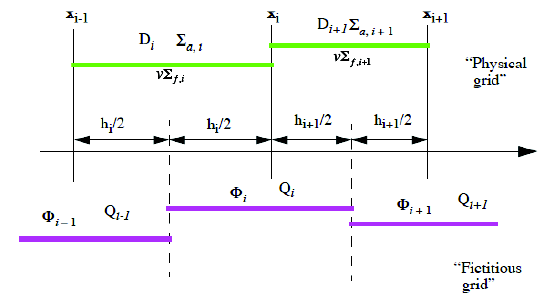
\includegraphics[height=2.5in]{FVM-eig-fig}
\end{figure}

We again assume the cross section and diffusion coefficient are constant in each cell 
\begin{align}
D(x) &= D_i\;, \qquad x_{i-1} \leq x \leq x_i \nonumber \\
\Sigma_a(x) &= \Sigma_{a,i}\;, \qquad x_{i-1} \leq x \leq x_i \nonumber \\
\nu\Sigma_f(x) &= \nu\Sigma_{f,i}\;, \quad x_{i-1} \leq x \leq x_i \nonumber \\
h_i &\equiv x_{i} - x_{i-1} \:.\nonumber 
\end{align}
%
We also still assume that the fluxes are constant over the interval centered around $x_i$:
%
\begin{align}
\phi(x) &= \phi_i \qquad \text{for } \bigl(x_i - \frac{h_i}{2}\bigr) \leq x \leq \bigl(x_i + \frac{h_{i+1}}{2}\bigr)\:. \nonumber %\\
%S(x) &= S_i \qquad \text{for } \bigl(x_i - \frac{h_i}{2}\bigr) \leq x \leq \bigl(x_i + \frac{h_{i+1}}{2}\bigr) \nonumber 
\end{align}

Now, we integrate the differential equation over each cell, $\bigl(x_i - \frac{h_i}{2}\bigr) \leq x \leq \bigl(x_i + \frac{h_{i+1}}{2}\bigr)$:
%
\[\int_{(x_i - \frac{h_i}{2})}^{(x_i + \frac{h_{i+1}}{2})} \biggl(  -\frac{d}{dx}D(x)\frac{d \phi(x)}{dx}\biggr) dx 
+ \int_{(x_i - \frac{h_i}{2})}^{(x_i + \frac{h_{i+1}}{2})} \Sigma_a(x) \phi(x) dx 
= \int_{(x_i - \frac{h_i}{2})}^{(x_i + \frac{h_{i+1}}{2})} \frac{1}{k}\nu \Sigma_f(x) \phi(x) dx\]
%
We'll only add the term we didn't do before:
%
\begin{align}
\int_{(x_i - \frac{h_i}{2})}^{(x_i + \frac{h_{i+1}}{2})} \frac{1}{k}\nu \Sigma_f(x)\phi(x) dx &= 
%
\int_{(x_i - \frac{h_i}{2})}^{(x_i)} \frac{1}{k}\nu \Sigma_f(x) \phi(x) dx + \int_{(x_i)}^{(x_i + \frac{h_{i+1}}{2})} \frac{1}{k}\nu \Sigma_f(x) \phi(x) dx \nonumber\\
%
&\nonumber \\
&= \frac{1}{k} \biggl(\frac{\nu\Sigma_{f,i}h_i + \nu\Sigma_{f,i+1}h_{i+1}}{2} \biggr)\phi_i \:.\nonumber 
\end{align}

Collecting all of the terms:
%
\begin{equation}
-D_{i+1}\biggl(\frac{\phi_{i+1} - \phi_i}{h_{i+1}}\biggr) + D_{i}\biggl(\frac{\phi_{i} - \phi_{i-1}}{h_{i}}\biggr) + \biggl(\frac{\Sigma_{a,i}h_i + \Sigma_{a,i+1}h_{i+1}}{2} \biggr)\phi_i =   \frac{1}{k} \biggl(\frac{\nu\Sigma_{f,i}h_i + \nu\Sigma_{f,i+1}h_{i+1}}{2} \biggr)\phi_i \:.\nonumber
\end{equation}

To express this in matrix form we'll use the same abbreviations as last time, and add one for the fission term (where we've divided through by $h_{ii}$ to get the x-sec terms):
\begin{align}
%h_{ii} &= \frac{h_i + h_{i+1}}{2} \nonumber \\
%%
%\Sigma_{a,ii} &= \frac{\Sigma_{a,i}h_i + \Sigma_{a,i+1}h_{i+1}}{h_i + h_{i+1}} \nonumber \\
\nu\Sigma_{f,ii} &= \frac{\nu\Sigma_{f,i}h_i + \nu\Sigma_{f,i+1}h_{i+1}}{h_i + h_{i+1}} \:.\nonumber
\end{align}
%
Then
%
\[a_{i,i-1} \phi_{i-1} + a_{i,i}\phi_i + a_{i, i+1} \phi_{i+1} = \frac{1}{k}\nu\Sigma_{f,ii} \phi_i \qquad \text{for } i = 1, 2, \dots, n-1\:,\]
%
where the $a$s have the same value as last time. (Only the rhs is new.)
%
%\begin{align}
%a_{i,i-1} &= \frac{-D_i}{h_i h_{ii}}\:, \nonumber \\
%a_{i,i} &= \frac{D_i}{h_i h_{ii}} + \frac{D_{i+1}}{h_{i+1} h_{ii}} +\Sigma_{a,ii}\:, \nonumber \\
%a_{i,i+1} &= \frac{-D_{i+1}}{h_{i+1} h_{ii}}:.\nonumber
%\end{align}

We again have a set of $n-1$ linear algebraic equations with $n+1$ unknowns. We will use the boundary conditions to get the rest of the information that we need.


%-------------------------------------------------------
\subsection*{Boundary Conditions}

Again assume $x_n = \tilde{a}$, then the \textbf{vacuum condition} becomes
\[\phi_n = 0\]
and the last equation for $i=n-1$ becomes
\[a_{n-1,n-2} \phi_{n-2} + a_{n-1,n-1}\phi_{n-1} + 0 = \frac{1}{k}\nu\Sigma_{f,(n-1,n-1)} \phi_{n-1}\]

To include the \textbf{reflecting} or zero current condition we integrate over $[0, h_{1}/2]$.
%
\begin{figure}[h!]
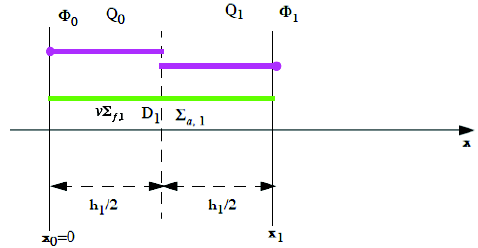
\includegraphics[height=2in]{ReflectingBC-eig}
\end{figure}
%
\begin{align}
\int_{0}^{\frac{h_{1}}{2}} \biggl(-\frac{d}{dx}D(x)\frac{d \phi(x)}{dx}\biggr) dx &+ \int_{0}^{\frac{h_{1}}{2}} \Sigma_a(x) \phi(x) dx = \int_{0}^{\frac{h_{1}}{2}} \frac{1}{k}\nu \Sigma_f(x) \phi(x) dx \:. \nonumber %\\
%
%-D(x)\frac{d \phi(x)}{dx}\big|_{\frac{h_{1}}{2}} &+ D(x)\frac{d \phi(x)}{dx}\big|_{0} + \Sigma_{a,1}\phi_0 \frac{h_1}{2} = \frac{1}{k}\nu\Sigma_{f,1} \phi_0 \frac{h_1}{2} \nonumber 
\end{align}
%
We perform the integration and can apply the boundary condition $\frac{d \phi(x)}{dx}\big|_{0} = 0$ just like last time, 
%\[-D(x)\frac{d \phi(x)}{dx}\big|_{\frac{h_{1}}{2}} + \Sigma_{a,1}\phi_0 \frac{h_1}{2} = \frac{1}{k}\nu\Sigma_{f,1} \phi_0 \frac{h_1}{2}\]
%%
%Recall that
%\[-D(x)\frac{d \phi(x)}{dx}\big|_{\frac{h_{1}}{2}} \cong -D_{1}\biggl(\frac{\phi_{1} - \phi_0}{h_{1}}\biggr) \]
%
and the first equation ($i=0$) becomes
\[a_{00}^*\phi_0 + a_{01}^* \phi_1 = \frac{1}{k}\nu\Sigma_{f,1} \phi_0 \:,\]
%
where we redefine the $a^*$s to be the same as last time as well.%to be (I've added the * to indicate that these have different definitions than the rest of the terms.)
%
%\begin{align}
%a_{00}^* &= \frac{2D_1}{h_1^2} + \Sigma_{a,1} \nonumber \\
%a_{01}^* &= -\frac{2D_1}{h_1^2} \nonumber 
%\end{align}

We now have $n$ equations and $n$ unknowns, but we formulate it a bit differently: 
\[\ve{A}\vec{\phi} = \frac{1}{k}\ve{F}\vec{\phi}\:,\]
where:
\begin{align}
%\ve{A} &= \begin{pmatrix}
%a_{00}^* & a_{01}^* & 0      & 0 & \cdots & 0 \\
%a_{10}   & a_{11}   & a_{12} & 0 & \cdots & 0 \\
%0        & a_{21}   & a_{22}   & a_{21} &  & \vdots \\
%\vdots        &    & \ddots  & \ddots & \ddots & \vdots \\
%0 & \cdots & 0 & a_{n-3,n-3}   & a_{n-2,n-2} & a_{n-2,n-1} \\
%0        & \cdots   & 0   & 0 & a_{n-1,n-2} & a_{n-1,n-1} 
%\end{pmatrix} \nonumber \\
%%
%\vec{\phi} &= \begin{pmatrix}\phi_0 \\ \phi_1 \\ \phi_2 \\ \vdots \\ \phi_{n-2} \\ \phi_{n-1} \end{pmatrix} \:, \qquad
%
\ve{F} = \begin{pmatrix}
\nu\Sigma_{f,1} & 0 & 0 & 0 & \cdots & 0 \\
0   & \nu\Sigma_{f,11} & 0  & 0 & \cdots & 0 \\
0   & 0 & \nu\Sigma_{f,22}  & 0 & \cdots & 0 \\
\vdots  &     & \ddots  & \ddots & \ddots  & \vdots \\
0 & \cdots & 0 & 0 & \nu\Sigma_{f,n-2,n-2} & 0 \\
0        & \cdots & 0 & 0   & 0 & \nu\Sigma_{f,n-1,n-1} 
\end{pmatrix} \:.\nonumber
\end{align}


%----------------------------------------------------------------
%----------------------------------------------------------------
\section*{Solution Methods}

We are only going to talk about iterative solution methods for eigenvalue problems since no one uses direct methods in practice (dealing with directly solving an eigenvalue matrix problem rapidly becomes intractable). We will formulate the problem this way
%
\[ \ve{A} \vec{\phi}^{(1)} = \frac{1}{k^{(0)}}\ve{F}\vec{\phi^{(0)}}\]

There are a variety of ways you can choose to determine convergence. We will consider these convergence criteria:
\begin{align}
\bigg|\frac{k^{(m)} - k^{(m-1)}}{k^{(m)}}\bigg| &< \epsilon_1 \:, \nonumber \\
\bigg|\frac{\phi_i^{(m)} - \phi_i^{(m-1)}}{\phi_i^{(m)}}\bigg| &< \epsilon_2 \qquad \forall i\:. \nonumber
\end{align}
%
Where $\epsilon_1$ is the eigenvalue convergence criterion (often $1 \times 10^{-4}$ or smaller), and $\epsilon_2$ is the flux error criterion (often $1 \times 10^{-3}$ or smaller).

\subsection*{Finding $k$}

But wait, that iterative method was only telling us how to update $\vec{\phi}$. How do we get new iterates for $k$? To sort that out, we're going to think about the physical interpretation of $k$.

The multiplication factor, $k$, can be defined as
\[k = \frac{\text{total production rate}}{\text{total loss rate}}\]
%
We can define two \textbf{operators} (\emph{not matrices}; to get the thing that we solve we apply our specific discretization methods to turn the operators into matrices) to help us compute this:
%
\begin{align}
A &= -\frac{d}{dx}D(x)\frac{d}{dx} + \Sigma_a(x) \quad \text{is the loss operator,} \nonumber \\
F &= \nu\Sigma_f(x) \qquad \qquad \text{is the production operator.}\nonumber
\end{align}

%Fortunately, the discretized versions of these operators are the matrices that we have $\ve{A}$ and $\ve{F}$, respectively. 
This allows us to write an equation for $k$ as
\[k^{(1)} = \frac{\int_0^{\tilde{a}} F \vec{\phi}^{(1)}(x)dx}{\int_0^{\tilde{a}} A \vec{\phi}^{(1)}(x)dx}\:. \]

We can express our iterative method with our operators,
\[ A \vec{\phi}^{(1)} = \frac{1}{k^{(0)}}F\vec{\phi^{(0)}}\]
%
and substitute this into our $k$ equation to get
\[k^{(1)} = \frac{\int_0^{\tilde{a}} F \vec{\phi}^{(1)}(x)dx}{\frac{1}{k^{(0)}}\int_0^{\tilde{a}} F \vec{\phi}^{(0)}(x)dx\:.} \]
%
This idea applies to any discretization strategy. To use the finite difference formulation we've developed, we discretize the operators and this can be expressed as:
\[k^{(1)} = k^{(0)}\Biggl(\frac{\nu\Sigma_{f,1} \phi_0^{(1)} \frac{h_1}{2} + \sum_{i=1}^{n-1} \nu\Sigma_{f,ii} \phi_i^{(1)} \frac{h_{ii}}{2}}
{\nu\Sigma_{f,1} \phi_0^{(0)} \frac{h_1}{2} + \sum_{i=1}^{n-1} \nu\Sigma_{f,ii} \phi_i^{(0)} \frac{h_{ii}}{2}}\Biggr)\:.\]

\subsection*{Power Method}

Power Iteration (PI) is an old and straightforward algorithm for finding an eigenvalue/vector pair. 

The basic idea is that any non-zero vector can be written as a linear combination of the eigenvectors of $\ve{B}$ because the eigenvectors are linearly independent, namely $v_0 = \gamma_1 x_1 + \gamma_2 x_2 + \cdots + \gamma_n x_n$, where $x_{j}$ is the $j$th eigenvector and $\gamma_{j}$ is some constant. This specific expression assumes a non-defective $\ve{B}$, though this assumption is not necessary for the method to work. 

Another fact that is used to understand power iteration is that $\ve{B}^m x_i = \lambda_i^m x_i$. Thus
%
\begin{equation}
  \ve{B}^m v_{0} = \gamma_1 \lambda_1^m x_1 + \gamma_2 \lambda_2^m x_2 + \cdots + \gamma_n \lambda_n^m x_n \:.\nonumber
  \label{eq:Ak}
\end{equation}
%
Since $|\lambda_1| > |\lambda_i|, i \ne 1$, the first term in the expansion will dominate as $k \to \infty$ and $\ve{B}^m v_{0}$ therefore becomes an increasingly accurate approximation to $x_1$. 

In practice, it is desirable to avoid exponentiating a matrix, so we will use an algorithm that does something else. It is also helpful to normalize $v_0$ to avoid possible over or underflow.

We are also quite interested in the \textit{convergence behavior} of PI. After $m$ steps, the iteration vector will be: 
%
\begin{equation}
  v_{m} = \bigl( \frac{\lambda_{1}^{m}}{e_{1}^{T}\ve{B}^{m}v_{0}} \bigr) \bigl(\frac{1}{\lambda_{1}^{m}}\ve{B}^{m}v_{0} \bigr) \:. \nonumber
\end{equation}
% 
If $\ve{B}$ has eigenpairs $\{(x_{j}, \lambda_{j}), 1 \le j \le n \}$ and $v_{0}$ has the expansion $v_{0} = \sum_{j=1}^{n} x_{j}\gamma_{j}$ then
%
\begin{equation}
  \frac{1}{\lambda_{1}^{m}}\ve{B}^{m}v_{0} =  \frac{1}{\lambda_{1}^{m}} \sum_{j=1}^{n} \ve{B}^{m}x_{j}\gamma_{j} = \sum_{j=1}^{n} x_{j} \bigl(\frac{\lambda_{j}}{\lambda_{1}} \bigr) \gamma_{j} \:.
  \label{eq:PIexpand}
\end{equation}
%
From equation \eqref{eq:PIexpand} it can be determined that the error is reduced in each iteration by a factor of $|\frac{\lambda_{2}}{\lambda_{1}}|$, which is called the dominance ratio. If $\lambda_2$ is close to $\lambda_1$, then this ratio will be close to unity and the method will converge very slowly. 

If $\lambda_2$ is far from $\lambda_1$, then convergence will happen much more quickly. Put simply, PI is better suited for problems where $\ve{B}$ has eigenvalues that are well separated.  

Power iteration is very attractive because it only requires matrix-vector products and two vectors of storage space. Because of its simplicity and low storage cost, PI has been widely used in the transport community for criticality problems for quite some time.

Despite these beneficial characteristics, many current codes use an acceleration method with PI or have moved away from it altogether because of the slow convergence for many problems of interest. Nevertheless, it is still used in some codes, has historical relevance, and is used in many studies as a base comparison case.


\subsubsection*{Algorithm}

The power method applies in our formulation when $\ve{B} \equiv \ve{A}^{-1}\ve{F}$, $\lambda \equiv k$ and $\vec{x} \equiv \vec{\phi}$. 
%
When we write it this way it is technically \textbf{inverse power iteration} because we're using the inverse of $\ve{A}$ rather than $\ve{A}$ (the theory is the same). Be careful when setting up these solvers about whether you are solving for $k$ or $1/k$ to ensure you get the correct eigenvectors.

Here is an algorithm to implement the power method (note: this is not the most efficient way to do this, but it is likely the clearest).
%
\begin{enumerate}
\item get initial values for $k^{(0)}$ and $\phi^{(0)}$ for $i = 0, \dots, n-1$; normalize $\phi_0 = \phi_0 / ||\phi_0||$

\item compute the elements of $\ve{A}$

\item compute the initial fission source
\[\vec{Q}_{f}^{(0)} = \begin{pmatrix}
Q_{f,0}^{(0)} \\ Q_{f,2}^{(0)} \\ \vdots \\ Q_{f,n-1}^{(0)} \\
\end{pmatrix}\]
%
where $Q_{f,i}^{(0)} = \nu\Sigma_{f,ii}\phi_i^{(0)} \: \text{for } i = 1, \dots, n-1$ and $Q_{f,0}^{(0)} = \nu\Sigma_{f,0}\phi_0^{(0)}$

\item for $m = 1, ...,$ convergence:
\begin{enumerate}
\item solve
\[\ve{A} \vec{\phi}^{(m)} = \frac{1}{k^{(m-1)}}\vec{Q}_{f}^{(m-1)}\]

\item compute the next fission source $\:Q_{f,i}^{(m)} = \nu\Sigma_{f,ii}\phi_i^{(m)} \: \text{ for } i = 1, \dots, n-1$ and\\ $Q_{f,0}^{(m)} = \nu\Sigma_{f,0}\phi_0^{(m)}$

\item compute the next eigenvalue:
\[k^{(m)} = k^{(m-1)}\Biggl(\frac{Q_{f,0}^{(m)} \frac{h_1}{2} + \sum_{i=1}^{n-1} Q_{f,i}^{(m)} \frac{h_{ii}}{2}}
{Q_{f,0}^{(m-1)} \frac{h_1}{2} + \sum_{i=1}^{n-1} Q_{f,i}^{(m-1)} \frac{h_{ii}}{2}}\Biggr)\]

\item check for convergence
\begin{align}
\bigg|\frac{k^{(m)} - k^{(m-1)}}{k^{(m)}}\bigg| &< \epsilon_1 \nonumber \\
\bigg|\frac{\phi_i^{(m)} - \phi_i^{(m-1)}}{\phi_i^{(m)}}\bigg| &< \epsilon_2 \nonumber
\end{align}

\end{enumerate}
\end{enumerate}

%--------------------------------------------------------------------
%--------------------------------------------------------------------
%\bibliographystyle{plain}
%\bibliography{LinearSolns} 

\end{document}